\chapter{Garment Segmentation}
\label{garment_segmentation}

This chapter is devoted to the first stage of our algorithm, segmenting the garment data from the whole sensor data. The input data is an RGB image with depth information (RGB-D image). Garment segmentation is perfomed over this image, and the garment contour is then extracted and simplified, ready to be used in later stages. \juansays{(Referenciar figura)}

\begin{figure}[thpb]
    \centering
    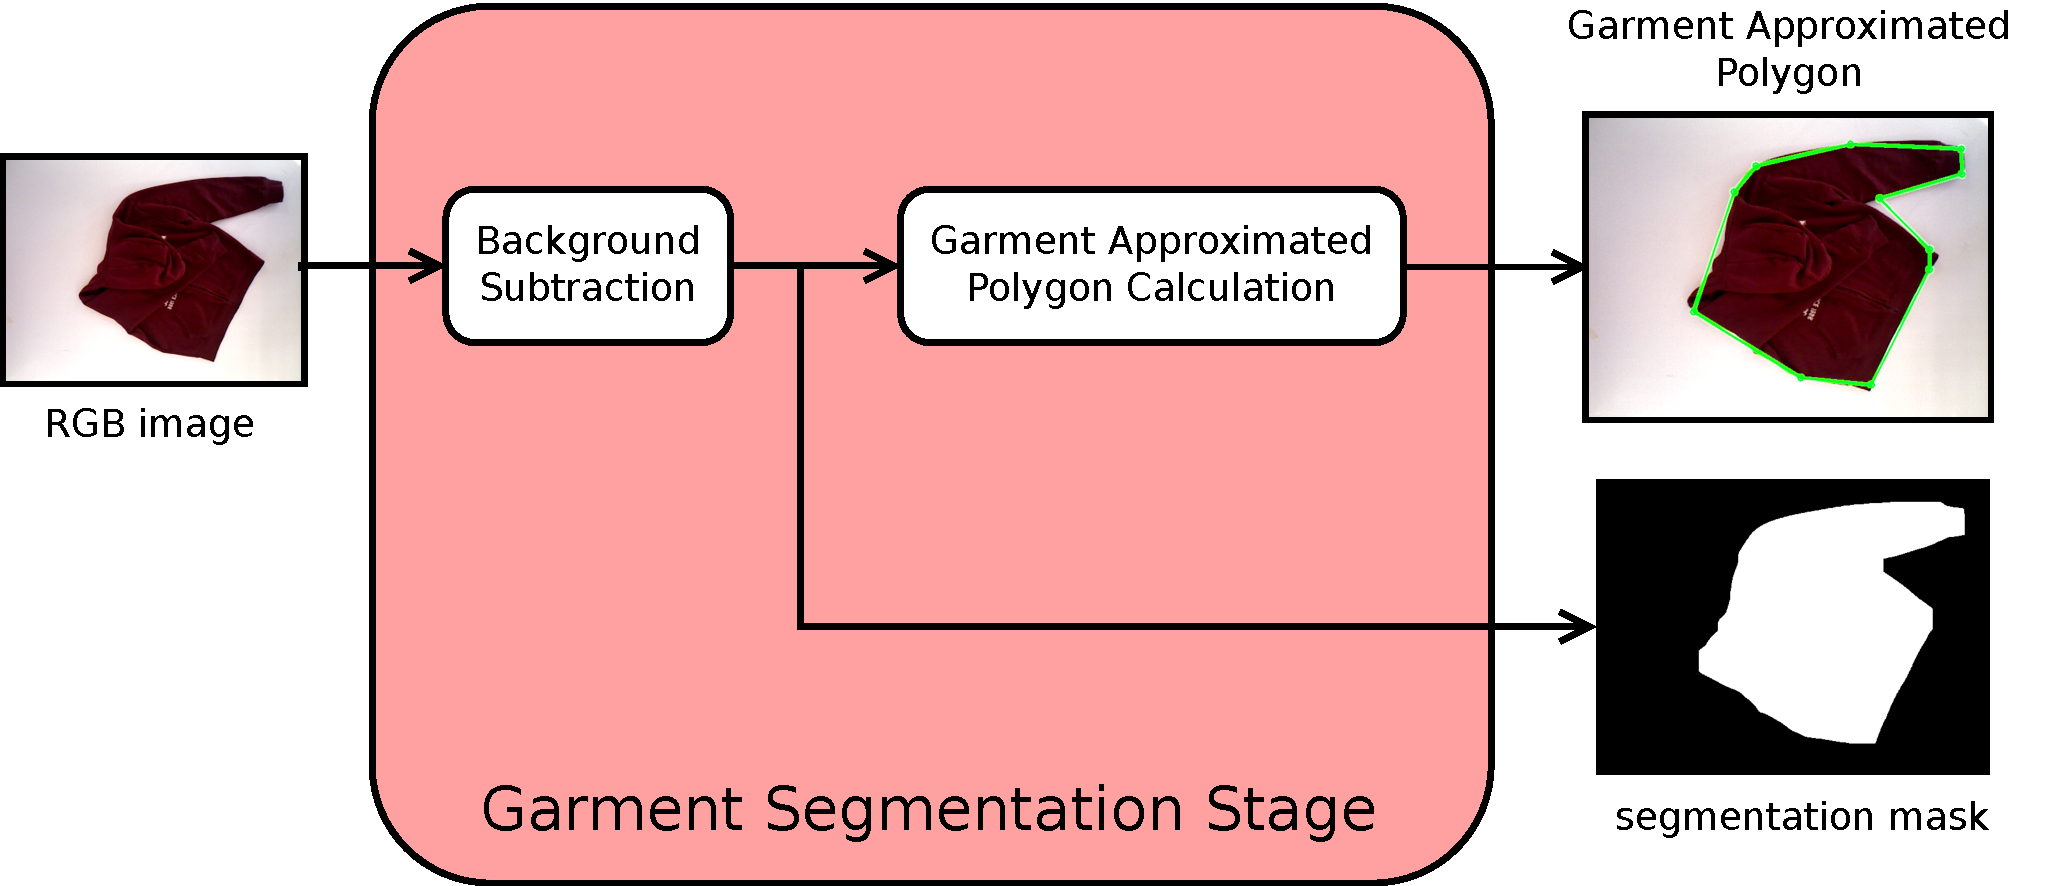
\includegraphics[width=\textwidth]
    {figures/Garment-segmentation-diagram.pdf}
    \caption{Block diagram showing an overview of the Garment Segmentation stage and its different steps. The input of this stage is an RGB image of the garment, and the outputs are the segmentation mask and the garment approximated polygon. The segmentation mask is also used as a by-product to obtain the approximated polygon.}
    \label{fig:garment_segmentation_blocks}
\end{figure}


\section{Background Subtraction}
\label{background_subtraction}

The RGB-D image obtained from the robot sensor contains both the clothing article and the table on which it rests. Therefore, after retrieving the data, a background subtraction step is required to classify whether a pixel represents the garment or the table. Figure \ref{fig:background_subtration_processes} shows an overview of the different processes involved in this step.


\begin{figure}[thpb]
    \centering
    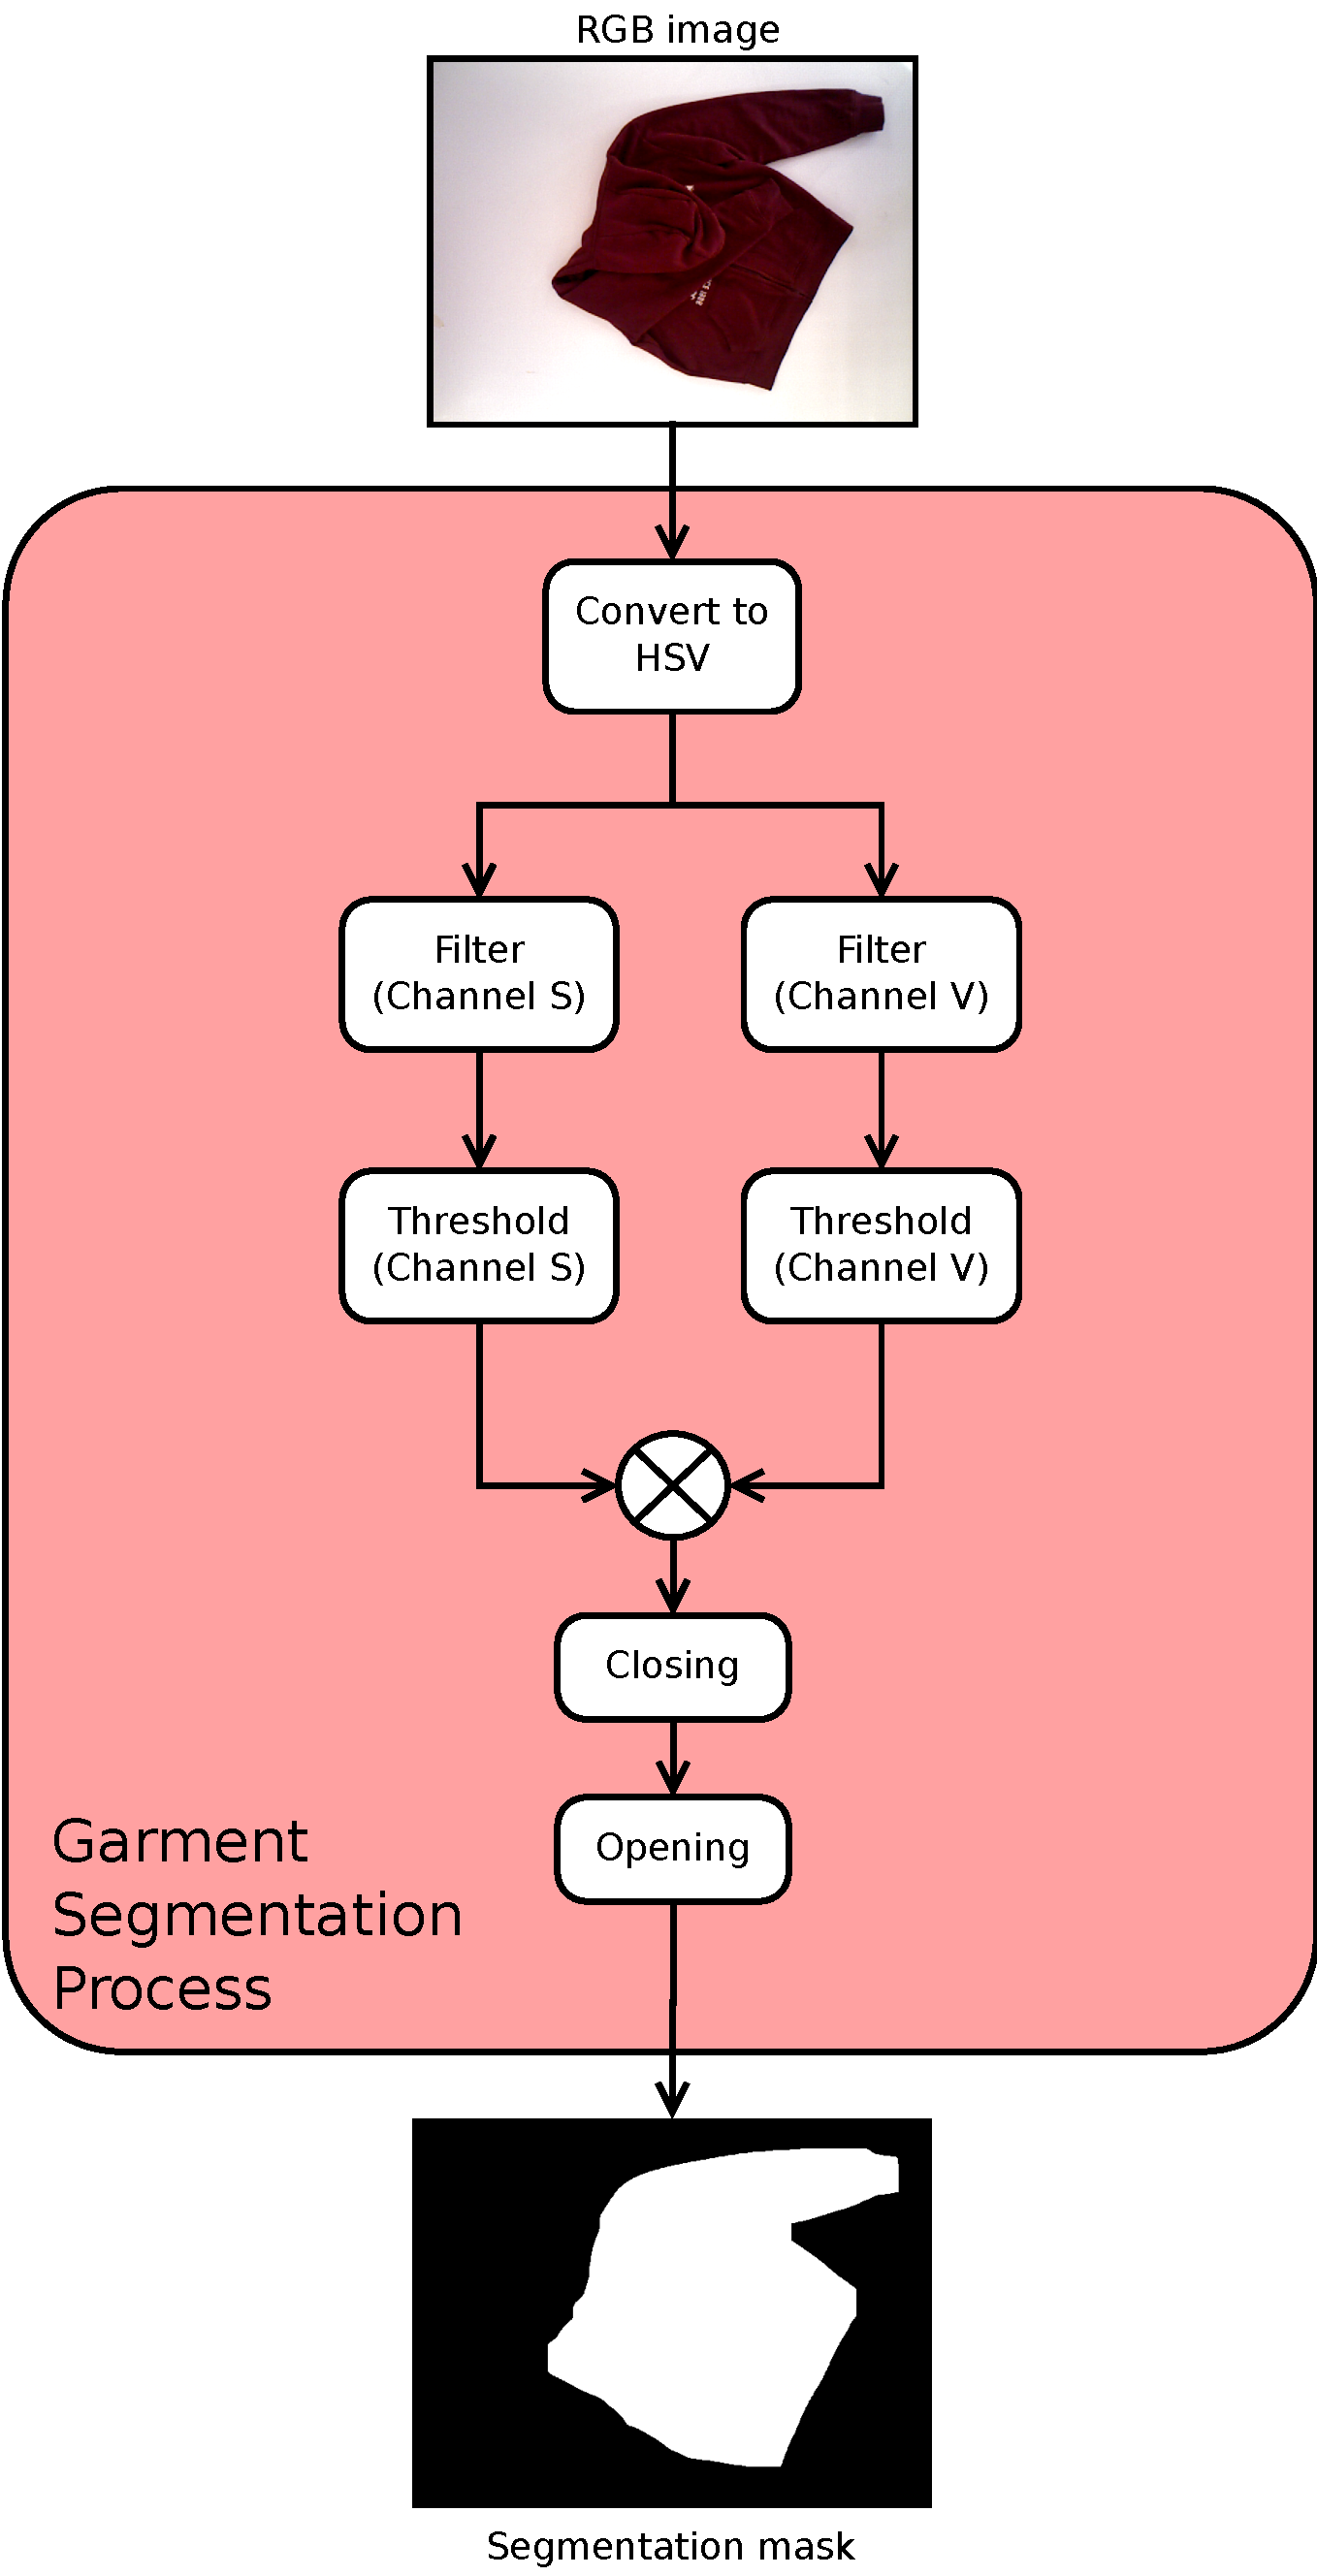
\includegraphics[width=0.6\textwidth]
    {figures/Garment-segmentation-process-diagram.pdf}
    \caption{Block diagram showing the different processes performed in the Garment Segmentation step. The left branch of the diagram corresponds to operations performed over the Saturation (S) channel, whereas the right branch of the diagram corresponds to operations over the Value (V) channel. The Hue (H) channel of the HSV image is not used. The results of the two threshold processes are merged together with a bitwise AND operation before applying the morphological operations.}
    \label{fig:background_subtration_processes}
\end{figure}

For this purpose, many methods could have been chosen, based on both color and depth information, as discussed in section \ref{architecture:garment_segmentation}. For instance, GrabCut \cite{rother2004grabcut} was discarded for background subtraction as it requires user input to select background and foreground samples. Furthermore, it is computationally expensive compared with simple thresholding methods. As the main focus of our work is unfolding clothes, a simple color-based method was selected instead. 


We work under the assumption that the garment has been placed over a flat white surface, as opposed to the garment which is much more colorful (higher Saturation). Therefore, the RGB image is converted to the HSV space. Working in the HSV space gives us direct information about our magnitudes of interest: Saturation (S) and Value (V). We are not interested in detecting a particular color, but to detect a colored item, so HSV is a more sensible choice of color space than RGB. 

A filtering process is added to increase robustness and reduce the effect of the noise on the background subtraction. This process is achieved using a convolution with a 5x5 and $\sigma=1.1$ Gaussian kernel computed on the Saturation and Value channels of the HSV image.

Once the image is converted to the HSV color space and filtered, a thresholding operation is then applied to the filtered image, using Otsu's algorithm \cite{otsu1975threshold} to obtain the optimal threshold values. Pixels with low amount of Saturation, and high Value are classified as being part of the table, as opposed to saturated or dark pixels.

Finally, some morphological transformations are applied to the resulting mask to reduce noise due to false positives/negatives. A 5x5 square kernel is used in several closing operations, followed by a similar number of opening operations. \juansays{"Ya veremos si explicarlo"}

The output of this background subtraction step, a binary mask with background pixels represented as black and garment pixels represented as white, can be seen in Figure \ref{fig:segmentation_mask}.

%\begin{figure}[thpb]
%    \centering
%    
\includegraphics[width=0.48
%    \textwidth]{figures/placeholder.png}
%    \caption{\comment{Again, I should put here a picture of the resulting mask}}
%    \label{fig:segmentation_mask}
%\end{figure}

\begin{figure}[htbp]
	\centering
    \begin{subfigure}[l]{0.49\textwidth}
	    \centering
    	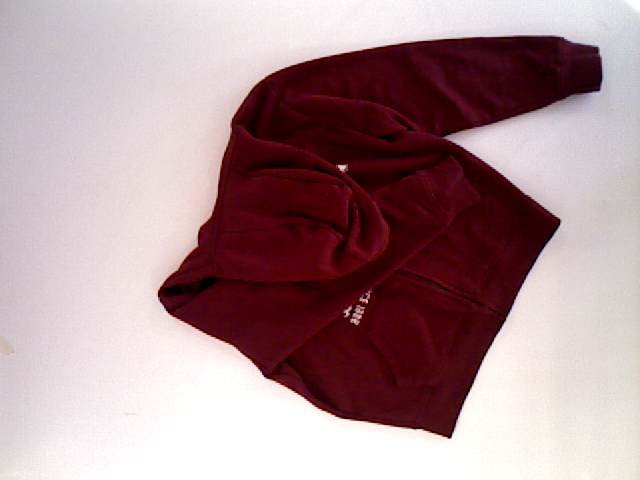
\includegraphics[width=\textwidth]
    	{figures/segmentation_original.png}
    	\caption{Original RGB image}
	\end{subfigure}
	~
    \begin{subfigure}[r]{0.49\textwidth}
	    \centering
    	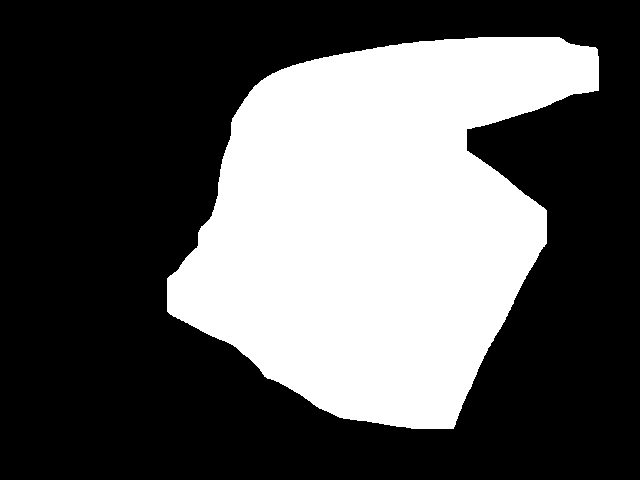
\includegraphics[width=\textwidth]
    	{figures/segmentation_mask.png}
    	\caption{Segmentation mask}
	\end{subfigure} 
    \caption{Original RGB image captured by the robot sensor versus the binary segmentation mask obtained after the background subtraction process. Black pixels represent the background, whereas white pixels represent pixels belonging to the garment.}
    \label{fig:segmentation_mask}
\end{figure}



\section{Garment Approximated Polygon Computation}
\label{segmentation_approximated_polygon}
From the binary mask obtained in the previous step (section \ref{background_subtraction}) a blob labeling algorithm is applied to detect the garment outline. This outline will be approximated to a simple polygon, and used in later stages to obtain the candidates to be a fold.

\begin{figure}[thpb]
    \centering
    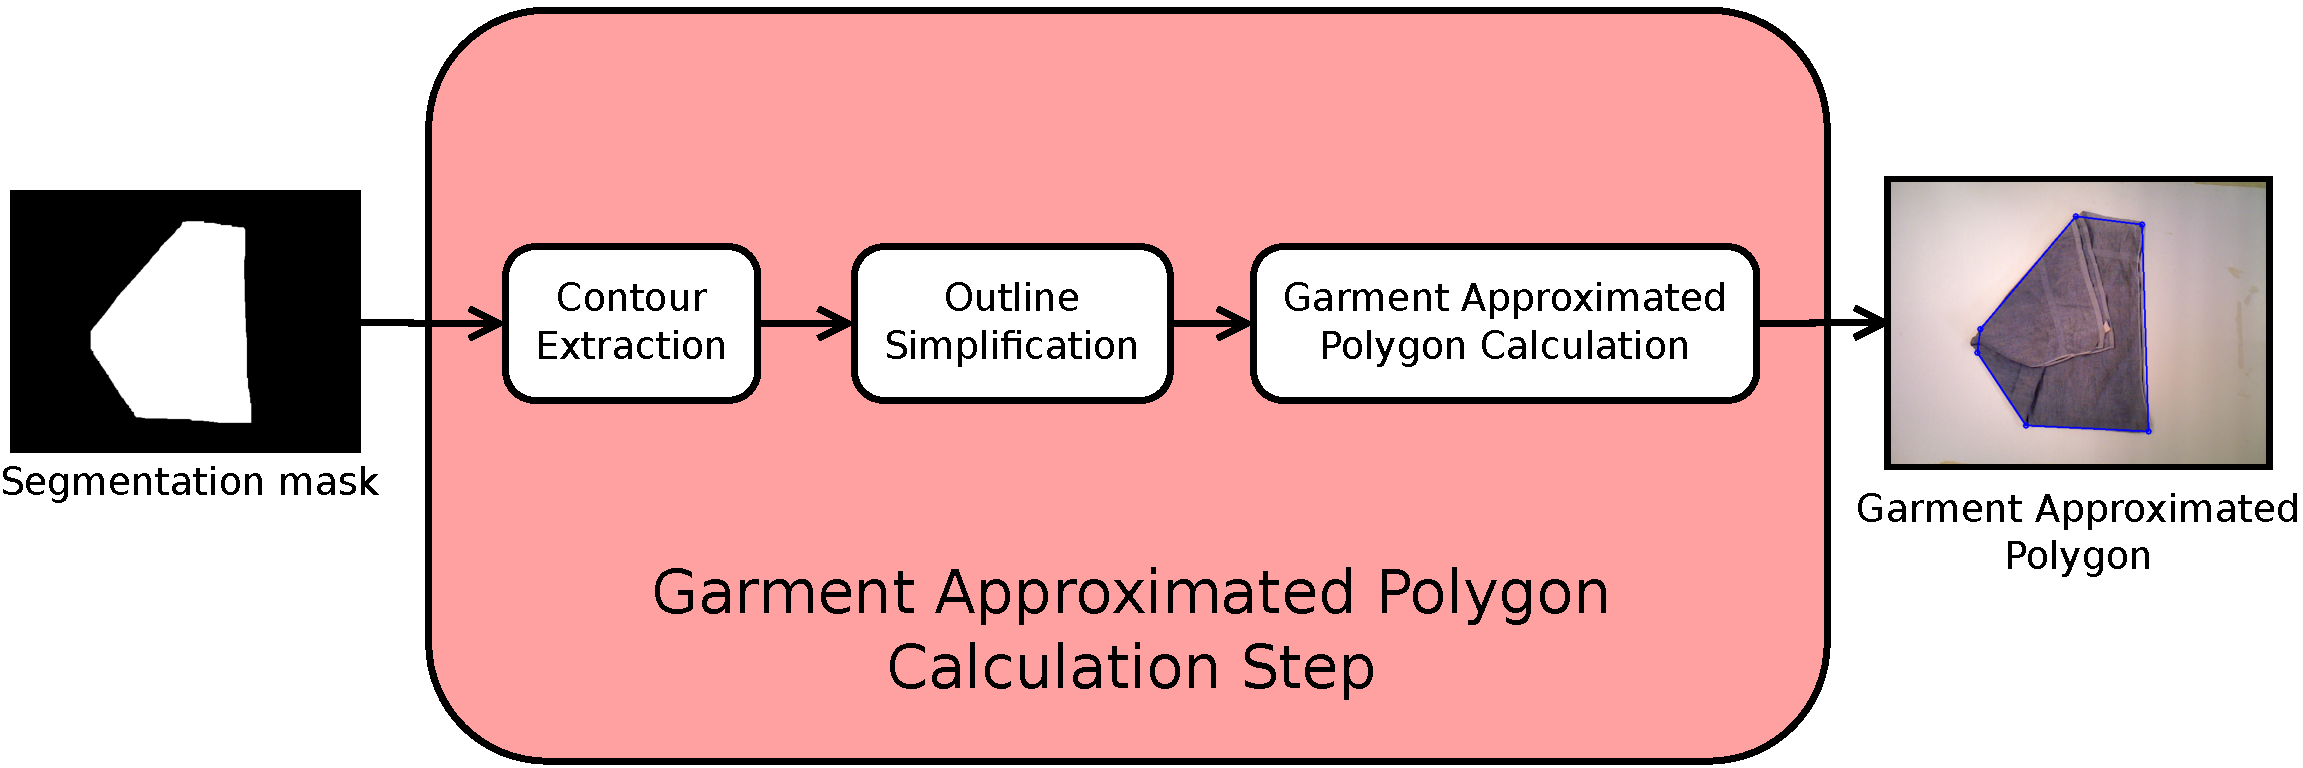
\includegraphics[width=\textwidth]
    {figures/Garment-polygon-diagram.pdf}
    \caption{Block diagram showing the different processes performed in the Garment Approximated Polygon Calculation step. The garment contour is obtained in the first process, and it is then simplified in the next processes to yield an Approximated Polygon that describes the garment.}
    \label{fig:garment_polygon_processes}
\end{figure}

The contour extraction method used is the Topological Analysis by Border Following algorithm developed by Suzuki and Abe \cite{suzuki1985topological}. It was selected as it is a widely used algorithm for connected-component labeling and countour finding. Other algorithms, such as Marching Cubes \cite{lorensen1987marching}, work under the assumption that contours are isolines\footnote{Curves along which a  function has a constant value.}, which is not the case for binary masks, so they are not suitable. Only external contours are retrieved. A simple chain approximation is then applied to reduce the number of points contained in the contours, storing only the endpoints of the different segments that describe the garment outline.

Due to noise, sometimes some small blobs appear in segmentation masks, so the outline with the largest area is selected as the garment outline. This way, those small blobs are discarded.

After obtaining the garment outline, it is futher processed, as we want to obtain a simplified description of the garment outline. This simplified description is the garment approximated polygon. We assume the fold line has a very high probability of lying in the garment polygon and, therefore, this polygon will represent all the candidate segments to be a fold. To obtain the approximated polygon, the Ramer–Douglas–Peucker algorithm \cite{ramer1972iterative, douglas1973algorithms} is applied. It is selected as it is efficient and a reliable implementation is available in the OpenCV\footnote{http://opencv.org/} libraries used to implement this work. This algorithm recursively divides the outline in segments by choosing the first and last points of the curve and drawing a line. Then, it checks whether that point is closer to that line than a threshold $\epsilon > 0$ or not. If it is closer, all points not marked to be kept can be discarded; otherwise, if it is greater than $\epsilon$, that point is marked to be kept and the procedure is repeated considering the last marked point as ending point. If there are no points left to process, the last point of the outline becomes the ending point again. The previous ending point becomes then the new starting point.

The parameter $\epsilon$ is calculated from the magnitude of the outline perimeter, considering it to be 1\% of that value. The greater this value is, the more simplified the resulting polygon will be.

Figure \ref{fig:contour_and_simplified_contour} shows a comparison between the garment contour, the garment outline and the final approximated polygon.

%\begin{figure}[thpb]
%    \centering
%    
\includegraphics[width=0.9
%    \textwidth]{figures/placeholder2.png}
%    \caption{\comment{Contour vs outline vs polygon}}
%    \label{fig:contour_and_simplified_contour}
%\end{figure}

\begin{figure}[htbp]
	\centering
    \begin{subfigure}[l]{0.49\textwidth}
	    \centering
    	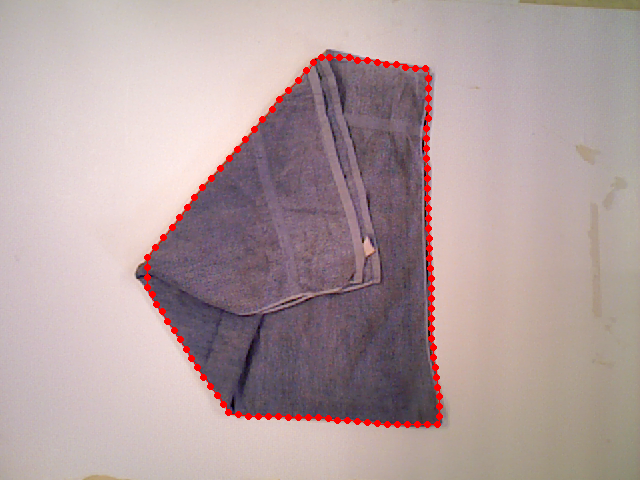
\includegraphics[width=\textwidth]
    	{figures/polygon-contour-01.png}
    	\caption{Garment Contour}
	\end{subfigure}
	~
    \begin{subfigure}[c]{0.49\textwidth}
	    \centering
    	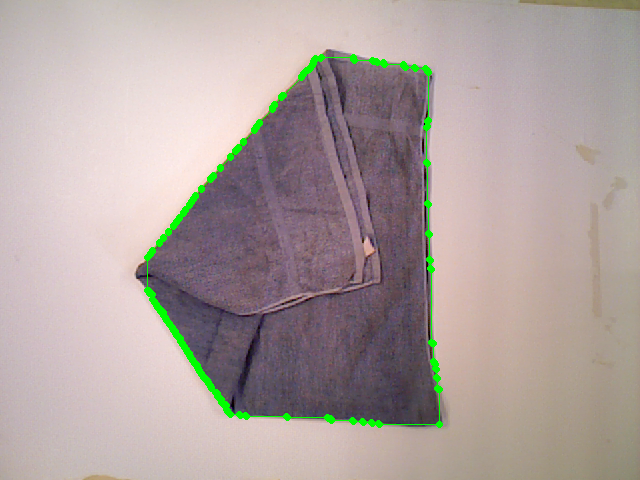
\includegraphics[width=\textwidth]
    	{figures/polygon-outline-01.png}
    	\caption{Garment Outline}
	\end{subfigure}
	~
    \begin{subfigure}[r]{0.49\textwidth}
	    \centering
    	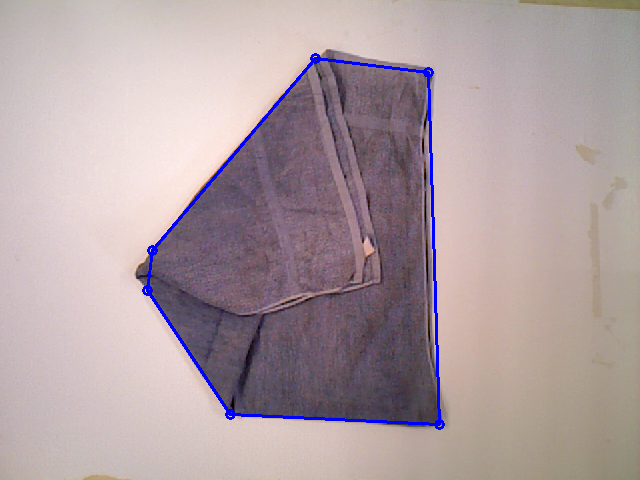
\includegraphics[width=\textwidth]
    	{figures/polygon-approx-01.png}
    	\caption{Garment Approximated Polygon}
	\end{subfigure} 
    \caption{Garment Contour, Garment Outline and Garment Appoximated Polygon. The Garment Contour contains all the points obtained from the segmentation mask. In the Garment Outline, points belonging to the same straight line are simplified and only the start and end points of the segment are used to represent it. After the Ramer-Douglas-Peucker algorithm is applied, a polygon with a low number of edges is obtained, which is used as Garment Approximated Polygon. }
    \label{fig:contour_and_simplified_contour}
\end{figure}
